
%(BEGIN_QUESTION)
% Copyright 2003, Tony R. Kuphaldt, released under the Creative Commons Attribution License (v 1.0)
% This means you may do almost anything with this work of mine, so long as you give me proper credit

When representing non-whole numbers, we extend the ``places'' of our decimal numeration system past the right of the decimal point, like this:

$$\includegraphics[width=15.5cm]{i02169x01.eps}$$

How do you suppose we represent non-whole numbers in a numeration system with a base (or ``radix") other than ten?  In the following examples, write the place-weight values underneath each place, and then determine the decimal equivalent of each example number:

\vskip 10pt

$$\includegraphics[width=15.5cm]{i02169x02.eps}$$

\vskip 20pt

$$\includegraphics[width=15.5cm]{i02169x03.eps}$$

\vskip 20pt

$$\includegraphics[width=15.5cm]{i02169x04.eps}$$

\underbar{file i02169}
%(END_QUESTION)





%(BEGIN_ANSWER)

$$\includegraphics[width=15.5cm]{i02169x05.eps}$$

\vskip 20pt

$$\includegraphics[width=15.5cm]{i02169x06.eps}$$

\vskip 20pt

$$\includegraphics[width=15.5cm]{i02169x07.eps}$$

%(END_ANSWER)





%(BEGIN_NOTES)

Many students will not realize initially that it is possible to represent non-whole numbers in binary, octal, or hexadecimal.  Really, though, the concept is identical to the representation of non-whole numbers in decimal form.  The ability of your students to grasp non-whole numbers in these other numeration systems indicates their grasp of place-weighted systems in general.  If a student truly comprehends how place-weighting works, they will have no trouble understanding digits to the left {\it or} the right of the radix point in any numeration system.  If a student does not understand how digits to the right of the decimal point are interpreted in other numeration systems, then they need to spend more time reviewing what decimal numbers mean.

It's not that the concept is so hard to understand, so much as it is our familiarity with the decimal (base-ten) numeration system.  We grow so accustomed to one way of representing numbers that we don't realize what the symbols actually {\it mean}, or that there may be alternative methods of representing quantities.

%INDEX% Electronics review: numeration system conversions

%(END_NOTES)


